\documentclass{article}
\usepackage{ctex}
\usepackage{float}
\usepackage{tikz}
\usetikzlibrary{shapes,arrows}
\tikzstyle{r} = [rectangle, minimum width=2cm, minimum height=1cm, text centered, draw=black]

\usepackage{enumerate}
\usepackage[a4paper,left=1cm,right=1cm,top=.5cm,bottom=.5cm]{geometry}
\usepackage{amsthm}
\usepackage{amsmath}
\theoremstyle{definition}
\newtheorem{question}{Question}
\newtheorem{answer}{Answer}
\newtheorem{subanswer}{answer}[answer]

\usepackage{etoolbox}
%\usepackage{enumitem}
%\newcommand*{\circled}[2][5]{
%	\lower.7ex\hbox{\tikz
%		\draw (0, 0) circle (.#1em)
%		node{\makebox[0cm][c]{\small #2}};
%		}
%	}
%\robustify{\circled}
	
	
\twocolumn

\title{人工智能作业}
\author{骆天奇\\2016254060407}
%\date{19.11.25}
\date{}
\begin{document}
	%\maketitle
	%\begin{question}
	假设已知下列事实:
	
	\begin{itemize}
		\item 小李(Li)喜欢容易的(Easy)程(Course)。
		\item 小李不喜欢难的(Difficult)课程。
		\item 工程类(Eng)课程都是难的。
		\item 物理类(Phy)课程都是容易的。
		\item 小吴(Wu)喜欢所有小李不喜欢的课程。
		\item Phy200是物理类课程。
		\item Eng300是工程类课程。
	\end{itemize}
	请用消解反演法回答下列问题:
	\begin{enumerate}
		\item 小李喜欢什么课程?
		\item 小吴喜欢Eng300课程吗?
	\end{enumerate}
\end{question}

\begin{question}
	某公司招聘工作人员,A,B,C三人应试,经面试后公司表示:
	\begin{itemize}
		\item 三人中至少录取一人
		\item 如果录取A而不录取B,则一定录取C
		\item 如果录取B,则一定录取C
	\end{itemize}
	问:公司一定录取谁?
\end{question}

	\begin{answer}
	\ \\
	\begin{tabular}{ll}
		\hline
		符号&定义\\
		\hline
		$Li$&小李\\
		$Wu$&小吴\\
		$C$&课程\\
		$Phy200$&一门物理课\\
		$Eng300$&一门工程课\\
		$Eng(C)$&课程C是工程课\\
		$Phy(C)$&课程C是物理课\\
		$Easy(C)$&课程C容易\\
		$Difficult(C)$&课程C难\\
		$Like(W,C)$&W喜欢课程C\\
		\hline
	\end{tabular}\\
	\paragraph{将事实化为子句}
	\begin{itemize}
		\item $(\forall C) (Easy(C) \rightarrow Like(Li,C))$
		\item $(\forall C) (Diffcult(C) \rightarrow \sim Like(Li,C))$
		\item $(\forall C) (Eng(C) \rightarrow Diffcult(C))$
		\item $(\forall C) (Phy(C) \rightarrow Easy(C))$
		\item $(\forall C) (\sim Like(Li,C) \rightarrow Like(Wu,C))$
		\item $Phy(Phy200)$
		\item $Eng(Eng300)$
	\end{itemize}
\begin{subanswer}\ \\
	公式集$S_1$
	\begin{align}
		& Eazy(C) \rightarrow Like(Li,C) \notag \\
		= & \sim Easy(C) \vee Like(Li,C)
		\end{align}
		\begin{align}
		& Phy(C) \rightarrow Easy(C) \notag \\
		= & \sim Phy(C) \vee East(C)
	\end{align}
	目标公式$L_2$
	\begin{equation}
		Like(Li, x) \label{math:l1}
	\end{equation}
	由问题得反演树
	\begin{figure}[H]
		\centering
		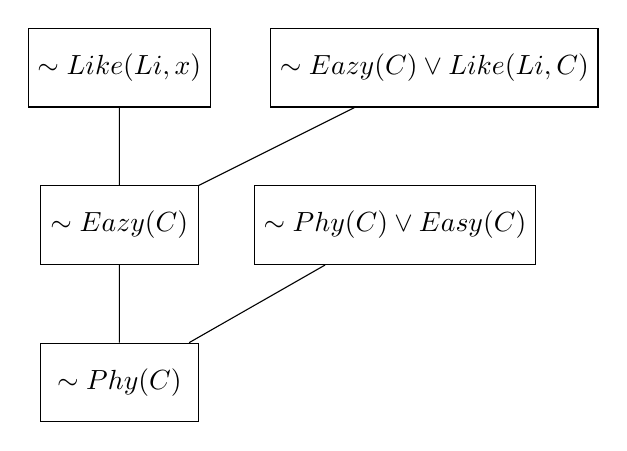
\begin{tikzpicture}[node distance=2cm]
			\node[r](1){$\sim Like(Li,x)$};
			\node[r,right of=1,xshift=2cm](2){$\sim Eazy(C) \vee Like(Li,C)$};
			\node[r,below of=1](3){$\sim Eazy(C)$};
			\node[r,right of=3,xshift=1.5cm](4){$\sim Phy(C)\vee Easy(C)$};
			\node[r,below of=3](5){$\sim Phy(C)$};
			\draw (1)--(3)--(2);
			\draw (3)--(5)--(4);
		\end{tikzpicture}
		\caption{反演树}
		\label{figure:1}
	\end{figure}
	\begin{enumerate}
		\item 目标公式(\ref{math:l1})否定的子句形式为
		\begin{equation}
			\sim Like(Li,x)
		\end{equation}
		将它添加至目标公式的否定之否定的子句中去,得重言式
		\begin{equation}
			\sim Like(Li,x) \vee Like(Li,x)
		\end{equation}
		\item 用图\ref{figure:1}的反演树进行消解得图\ref{figure:2},并在根节点得到子句
		\begin{equation}
			\sim Phy(C) \vee Like(Li,C)\label{math:res1}
		\end{equation}
		\item 求得答案,语句(\ref{math:res1})作为回答语句
		\item 小李喜欢物理课
	\end{enumerate}
	\begin{figure}[H]
		\centering
		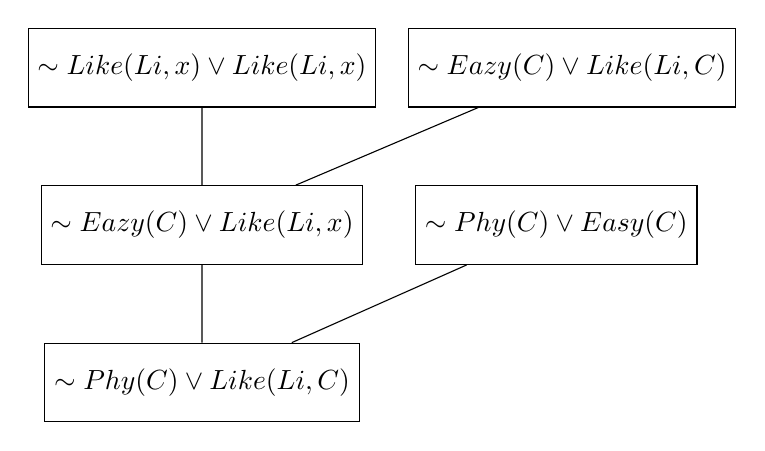
\begin{tikzpicture}[node distance=2cm]
		\node[r](1){$\sim Like(Li,x) \vee Like(Li,x)$};
		\node[r,right of=1,xshift=2.7cm](2){$\sim Eazy(C) \vee Like(Li,C)$};
		\node[r,below of=1](3){$\sim Eazy(C) \vee Like(Li,x)$};
		\node[r,right of=3,xshift=2.5cm](4){$\sim Phy(C)\vee Easy(C)$};
		\node[r,below of=3](5){$\sim Phy(C) \vee Like(Li,C)$};
		\draw (1)--(3)--(2);
		\draw (3)--(5)--(4);
		\end{tikzpicture}
		\caption{求取答案反演树}
		\label{figure:2}
	\end{figure}
\end{subanswer}
\begin{subanswer}\ \\
	公式集$S_2$
	\begin{align}
	& Diffcult(C) \rightarrow \sim Like(Li,C) \notag \\
	= & \sim Difficult(C) \vee \sim Like(Li,C)
	\end{align}
	\begin{align}
	& Eng(C) \rightarrow Diffcult(C) \notag \\
	= & \sim Eng(C) \vee Diffcult(C)
	\end{align}
	\begin{align}
	&\sim Like(Li,C) \rightarrow Like(Wu,C) \notag \\
	= &\sim \sim Like(Li,C) \vee Like(Wu,C) \notag \\
	= & Like(Li,C) \vee Like(Wu,C)
	\end{align}
	\begin{align}
	&Eng(Eng300)
	\end{align}
	目标公式$L_2$
	\begin{equation}
	Like(Wu,x) \label{math:l2}
	\end{equation}
	由问题得反演树
	\begin{figure}[H]
		\centering
		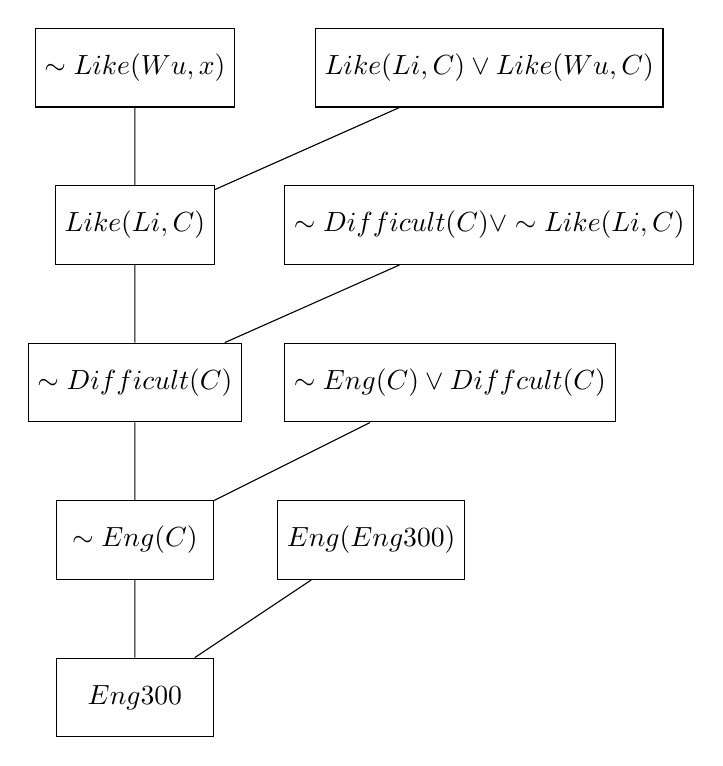
\begin{tikzpicture}[node distance=2cm]
		\node[r,xshift=1cm](1){$\sim Like(Wu,x)$};
		\node[r,right of=1,xshift=2.5cm](2){$Like(Li,C) \vee Like(Wu,C)$};
		\node[r,below of=1](3){$Like(Li,C)$};
		\node[r,right of=3,xshift=2.5cm](4){$\sim Difficult(C) \vee \sim Like(Li,C)$};
		\node[r,below of=3](5){$\sim Difficult(C)$};
		\node[r,right of=5,xshift=2cm](6){$\sim Eng(C) \vee Diffcult(C)$};
		\node[r,below of=5](7){$\sim Eng(C)$};
		\node[r,right of=7,xshift=1cm](8){$Eng(Eng300)$};
		\node[r,below of=7](9){$Eng300$};
		
		\draw (1)--(3)--(2);
		\draw (3)--(5)--(4);
		\draw (5)--(7)--(6);
		\draw (7)--(9)--(8);
		\end{tikzpicture}
		\caption{反演树}
		\label{figure:3}
	\end{figure}
	\begin{enumerate}
		\item 目标公式(\ref{math:l2})否定的子句形式为
		\begin{equation}
			\sim Like(Wu,x)
		\end{equation}
		将它添加至目标公式的否定之否定的子句中去,得重言式
		\begin{equation}
			\sim Like(Wu,x) \vee Like(Wu,x)
		\end{equation}
		\item 用图\ref{figure:3}的反演树进行消解得图\ref{figure:4},并在根节点得到子句
		\begin{eqnarray}
			Like(Wu,Eng300) \label{math:res2}
		\end{eqnarray}
		\item 得到答案,语句(\ref{math:res2})作为回答语句
		\item 小吴喜欢Eng300
		\begin{figure}[H]
			\centering
			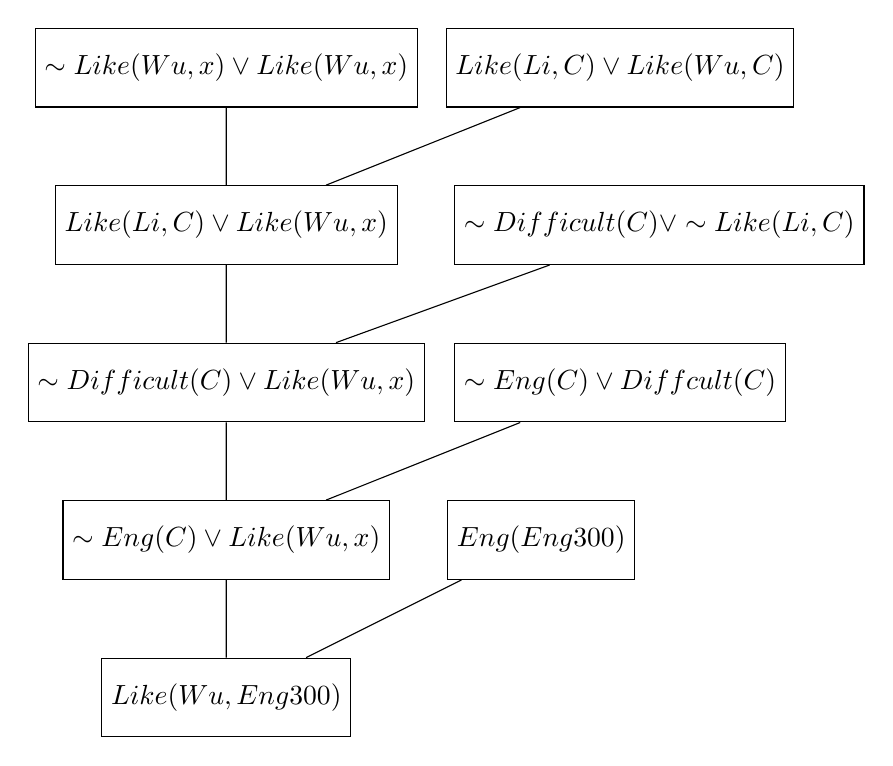
\begin{tikzpicture}[node distance=2cm]
			\node[r,xshift=1cm](1){$\sim Like(Wu,x) \vee Like(Wu,x)$};
			\node[r,right of=1,xshift=3cm](2){$Like(Li,C) \vee Like(Wu,C)$};
			\node[r,below of=1](3){$Like(Li,C) \vee Like(Wu,x)$};
			\node[r,right of=3,xshift=3.5cm](4){$\sim Difficult(C) \vee \sim Like(Li,C)$};
			\node[r,below of=3](5){$\sim Difficult(C) \vee Like(Wu,x)$};
			\node[r,right of=5,xshift=3cm](6){$\sim Eng(C) \vee Diffcult(C)$};
			\node[r,below of=5](7){$\sim Eng(C) \vee Like(Wu,x)$};
			\node[r,right of=7,xshift=2cm](8){$Eng(Eng300)$};
			\node[r,below of=7](9){$Like(Wu,Eng300)$};
			
			\draw (1)--(3)--(2);
			\draw (3)--(5)--(4);
			\draw (5)--(7)--(6);
			\draw (7)--(9)--(8);
			\end{tikzpicture}
			\caption{求取答案反演树}
			\label{figure:4}
		\end{figure}
	\end{enumerate}
\end{subanswer}
\end{answer}
\begin{answer}
	\ \\
	\begin{tabular}{ll}
		\hline
		符号&定义\\
		\hline
		A&录取A\\
		B&录取B\\
		C&录取C\\
		R&录取任意人\\
		\hline
	\end{tabular}
	\\
	\paragraph{将事实化为子句}
	\begin{itemize}
		\item $A \vee B \vee C$
		\item $(A \wedge \sim B) \rightarrow C$
		\item $B \rightarrow C$
	\end{itemize}
	公式集$S_3$
	\begin{align}
		A \vee B \vee C
	\end{align}
	\begin{align}
		&(A \wedge \sim B) \rightarrow C \notag \\
		= &\sim (A \wedge \sim B) \vee C \notag \\
		= &(\sim A \vee \sim \sim B) \vee C \notag \\
		= & \sim A \vee B \vee C
	\end{align}
	\begin{align}
		& B \rightarrow C \notag \\
		= & \sim B \vee C
	\end{align}
	目标公式$L_3$
	\begin{equation}
		A \vee B \vee C \label{math:l3}
	\end{equation}
	由问题得反演树
	\begin{figure}[H]
		\centering
		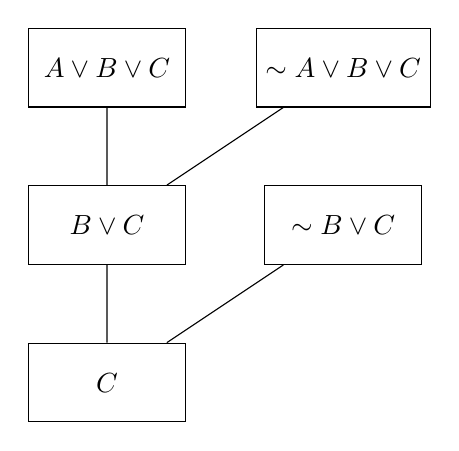
\begin{tikzpicture}[node distance=2cm]
		\node[r,xshift=1cm](1){$A \vee B \vee C$};
		\node[r,right of=1,xshift=1cm](2){$\sim A \vee B \vee C$};
		\node[r,below of=1](3){$B \vee C$};
		\node[r,right of=3,xshift=1cm](4){$\sim B \vee C$};
		\node[r,below of=3](5){$C$};
		
		\draw (1)--(3)--(2);
		\draw (3)--(5)--(4);
		\end{tikzpicture}
		\caption{反演树}
		\label{figure:5}
	\end{figure}
	\begin{enumerate}
		\item 通过图\ref{figure:5}反演树的根节点得子句
		\begin{equation}
			C \label{math:res3}
		\end{equation}
	\item 得到答案,语句(\ref{math:res3})作为回答语句
	\item 公司一定录取C
\end{enumerate}
\end{answer}
% 曲线救国
\paragraph{\ \ \ \ 信息与计算科学\ 骆天奇\ 2016254060407}
\end{document}
